\chapter{Practical examples}\label{chap:chap4}

All the examples presented here are drawn from Infer.NET's tutorial
\cite{InferNET14t}

\section{Two coins}

This example is a simple one, where we want to first determine the probability of
two coins being heads, and then say that the two weren't heads and ask for the
probability of the first one being heads.
We can see the resulting representation in Figure \ref{fig:firstExample}, which generates the following code:

\begin{lstlisting}
  using System;
  using System.Collections.Generic;
  using System.Text;
  using MicrosoftResearch.Infer.Models;
  using MicrosoftResearch.Infer;

  namespace Examples
  {
  	public class FirstExample
  	{
  		public void Run()
  		{
  			InferenceEngine engine = new InferenceEngine();
  			engine.Algorithm = new ExpectationPropagation();
        Variable<bool> firstCoin;
  			Variable<bool> secondCoin;
  			Variable<bool> bothHeads;

  			firstCoin = Variable.Bernoulli(0.5);
        secondCoin = Variable.Bernoulli(0.5);
        bothHeads = (firstCoin & secondCoin);

        if (!(ie.Algorithm is VariationalMessagePassing)) {
  				Console.WriteLine(String.concat("Probability both coins are heads: ", ie.Infer(bothHeads));
  				bothHeads.ObservedValue = false;
  				Console.WriteLine(String.concat("Probability distribution over firstCoin: ", ie.Infer(firstCoin));
  			} else {
  				Console.WriteLine("This example does not run with Variational Message Passing");
    		}
  	}
  }
\end{lstlisting}

In this fairly simple example we represent some of the most important semantics
of a PPL: declaring random variables, the dependicies between them and plugging
in observed values. In the next examples we will be adding more constructs on
top of these basic ones, so the reader can be convinced that this representation
is easily extensible.

\begin{figure}[t]
  \begin{center}
    \leavevmode
    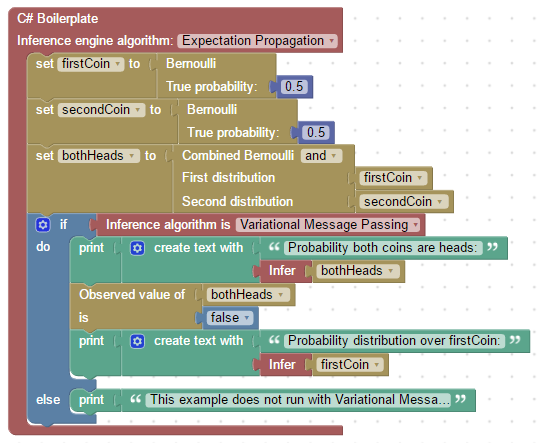
\includegraphics[width=0.86\textwidth]{firstExample}
    \caption{First example of a PP with our Blockly-powered VPE.}
    \label{fig:firstExample}
  \end{center}
\end{figure}

\section{Truncated Gaussian}

In this example, we define a Gaussian distribution and then query for the
result of that distribution when we restrict its values to be greater than a
certain threshold. The generated code is below, while the graphical representation
is in \ref{fig:truncatedGaussian}.

\begin{lstlisting}
using System;
using System.Collections.Generic;
using System.Text;
using MicrosoftResearch.Infer.Models;
using MicrosoftResearch.Infer;
using MicrosoftResearch.Infer.Distributions;
using MicrosoftResearch.Infer.Maths;

namespace BlocklyInfer
{
	public class BlocklyInfer
	{
		public static void Main()
		{
			InferenceEngine engine = new InferenceEngine();
			engine.Algorithm = new ExpectationPropagation();
			dynamic thresh;
			Variable<double> x;


			for (thresh = 0; thresh <= 1; thresh += 0.1) {
			    x = (Variable.GaussianFromMeanAndVariance(0, 1));
			    Variable.ConstrainTrue((x > thresh));
			    if (engine.Algorithm is ExpectationPropagation) {
			      Console.WriteLine(String.Concat("Dist over x given thresh of ", thresh, "=", (engine.Infer(x))));
			    } else {
			      Console.WriteLine("This example only runs with Expectation Propagation");
			    }

			  }
		}
	}
}
\end{lstlisting}

\begin{figure}[t]
  \begin{center}
    \leavevmode
    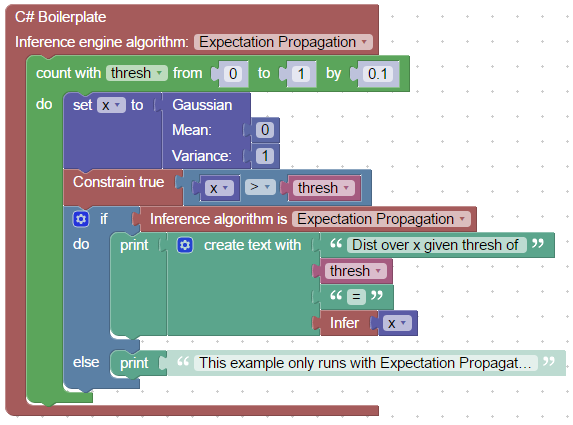
\includegraphics[width=0.86\textwidth]{truncatedGaussian}
    \caption{Truncated Gaussian PP}
    \label{fig:truncatedGaussian}
  \end{center}
\end{figure}

There is yet another version similar to the first one, but where we use a random
variable to represent a number rather than a normal number, which leads to a more
efficient inference process. This shows how Blockly's type system is good
enough to be strict but also flexible; in this case, the observedValue function
can either receive numbers or random numbers as part of the input. The code is shown
below and is generated from the model of Figure \ref{fig:truncatedGaussianEfficient}.

\begin{lstlisting}
using System;
using System.Collections.Generic;
using System.Text;
using MicrosoftResearch.Infer.Models;
using MicrosoftResearch.Infer;
using MicrosoftResearch.Infer.Distributions;
using MicrosoftResearch.Infer.Maths;

namespace BlocklyInfer
{
	public class BlocklyInfer
	{
		public static void Main()
		{
			InferenceEngine engine = new InferenceEngine();
			engine.Algorithm = new ExpectationPropagation();
			dynamic thresh;
			Variable<double> threshold;
			Variable<double> x;


			threshold = (Variable.New<double>());
			  x = (Variable.GaussianFromMeanAndVariance(0, 1));
			  Variable.ConstrainTrue((x > threshold));
			  if (engine.Algorithm is ExpectationPropagation) {
			    for (thresh = 0; thresh <= 1; thresh += 0.1) {
			      threshold.ObservedValue = thresh;
			      Console.WriteLine(String.Concat("Dist over x given thresh of ", thresh, "=", (engine.Infer(x))));
			    }
			  } else {
			    Console.WriteLine("This example only runs with Expectation Propagation");
			  }
		}
	}
}
\end{lstlisting}

\begin{figure}[t]
  \begin{center}
    \leavevmode
    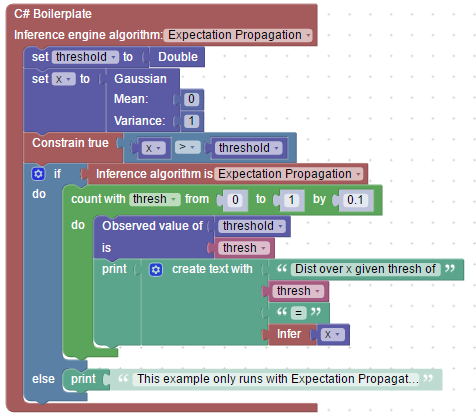
\includegraphics[width=0.86\textwidth]{truncatedGaussianEfficient}
    \caption{Truncated Gaussian written more efficiently PP}
    \label{fig:truncatedGaussianEfficient}
  \end{center}
\end{figure}

These examples are an extension of the first one with added loop constructs,
the possibility of defining a single random number and the possibility to constrain
numeric distributions.

\section{Learning a Gaussian}

In this model, we're trying to infer the mean and precision of a given dataset
(generated randomly). The most distiguishing aspect of this example is that it
deals with lists. The resulting code from the model of Figure \ref{fig:learningAGaussian}
is shown below.

\begin{lstlisting}
using System;
using System.Collections.Generic;
using System.Text;
using MicrosoftResearch.Infer.Models;
using MicrosoftResearch.Infer;
using MicrosoftResearch.Infer.Distributions;
using MicrosoftResearch.Infer.Maths;

namespace BlocklyInfer
{
	public class BlocklyInfer
	{
		public static void Main()
		{
			InferenceEngine engine = new InferenceEngine();
			engine.Algorithm = new ExpectationPropagation();
			dynamic dataLength;
			dynamic data;
			dynamic i;
			Variable<double> mean;
			Variable<double> precision;
			Variable<double> x;


			dataLength = 100;
			  data = new List<dynamic> {};
			  for (var count = 0; count < dataLength; count++) {
			    data.Add((Rand.Normal(0, 1)));
			  }
			  mean = (Variable.GaussianFromMeanAndVariance(0, 100));
			  precision = (Variable.GammaFromShapeAndScale(1, 1));
			  var i_end = dataLength - 1;
			  var i_inc = 1;
			  if (0 > i_end) {
			    i_inc = -i_inc;
			  }
			  for (i = 0;
			       i_inc >= 0 ? i <= i_end : i >= i_end;
			       i += i_inc) {
			    x = (Variable.GaussianFromMeanAndPrecision(mean, precision));
			    x.ObservedValue = (data[i]);
			  }
			  Console.WriteLine(String.Concat("mean=", engine.Infer(mean)));
			  Console.WriteLine(String.Concat("precision=", engine.Infer(precision)));
		}
	}
}
\end{lstlisting}

This is the longest generated code of all the examples, and the reason why the
second loop looks so different from the one that would be written by a programmer
is a consequence of using a variable (dataLength) in a loop where we want to
re-use the variable used to count the loop's iterations. If you look at the
operations before the second loop, you can notice that they exist because they
give the flexibility to the user of looping in the reverse order. Aside from
this, the example is yet another natural extension of the first one, where we
added more types of distributions.

\begin{figure}[t]
  \begin{center}
    \leavevmode
    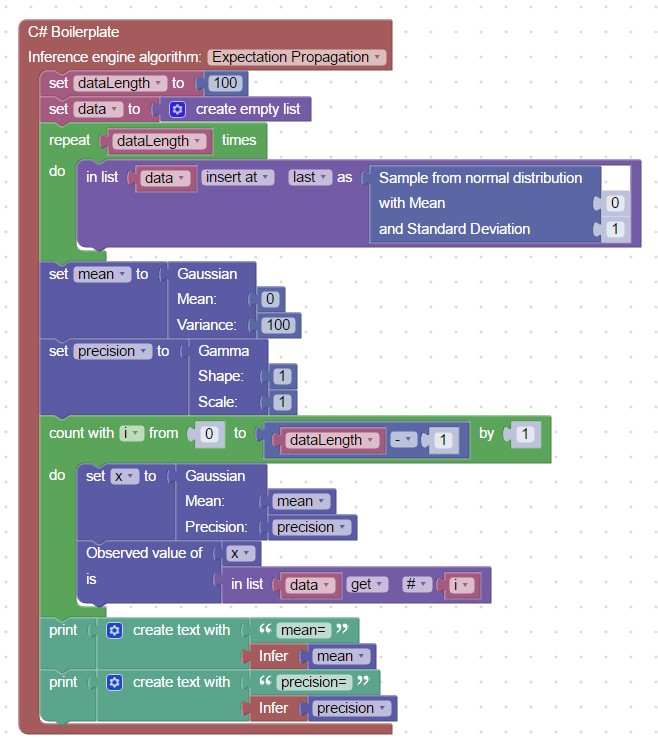
\includegraphics[width=0.86\textwidth]{learningAGaussian}
    \caption{Learning a Gaussian distribution}
    \label{fig:learningAGaussian}
  \end{center}
\end{figure}

\section{Conclusions}

The generated code is fairly similar to one that a human would
write, with the exceptions of string concatenation (in this case it would be more natural
to join the text with the inference result via the plus operator rather than
using String.concat), variables being declared and set in different lines and some
types of loops (which have been justified in the last example).

It is our belief that the graphical representation is clearar than its textual
counterpart, mainly because parameters are named (it is clear that 0.5 is the
probability of true when defining a Bernoulli distributions) and due to the use
of colors: red for statements related with
the inference engine, dark yellow for boolean distributions, green for text
and I/O, blue for booleans and control structures and purple for numbers.
